\documentclass[12pt]{article}

\usepackage{geometry}
\usepackage{amsmath,amsthm,amssymb}
\usepackage{graphicx}
\usepackage{multicol}

\newcommand{\lemma}{\noindent \textbf{Lemma: }}
\newcommand{\thm}{\noindent \textbf{Theorem: }}
\newcommand{\lskip}{\vspace{\baselineskip}}

\begin{document}

\title{Red-Black and 2-3-4 Trees}
\author{}
\maketitle

\section*{Description}
Red-black trees are loosely self-balanced BSTs. They have a 1-to-1 correspondence to 2-3-4 trees, and are easier and more efficient to implement; however, the theory behind the rebalancing is clearer to illustrate with 2-3-4 trees.

Compared to AVL trees, lookup times in a red-black tree are generally slower because they are less strictly balanced. However, insertion and deletion are generally faster because they require fewer rotations to rebalance the tree. In general red-black trees are used for language libraries (e.g. C++'s set and map) and AVL trees are used in databases, where fast lookups are preferred.

\section*{Properties}
2-3-4 trees have the following properties:
\begin{enumerate}
  \item Each node has either 2, 3, or 4 children (and 1 fewer key). \item The depth of every leaf node is the same.
\end{enumerate}

\noindent Red-black trees have the following properties.
\begin{enumerate}
  \item Nodes are colored red or black.
  \item The root is always black.
  \item No red node has a red child.
  \item \label{rb_desc_prop} Every path from a given node to each of its descendant leaves has the same number of black nodes.
\end{enumerate}
Note that by Property \ref{rb_desc_prop}, every root-to-leaf path has the same number of black nodes. We refer to this value as the \emph{black height} of the tree. The black height of a red-black tree is equal to the height of its corresponding 2-3-4 tree.

\section*{Insertion}
To insert into a red-black tree, we start with a normal BST insert and color the inserted node $N$ red. There are three cases for the position of $N$.
\begin{enumerate}
  \item $N$ is the root. In this case, we just color the insertednode the black and we have increase the black height of the tree by 1.
  \item $N$ has a black parent. In this case, the black height has not changed and no double red was created, so we are done.
  \begin{figure}[h!]
    \centering
    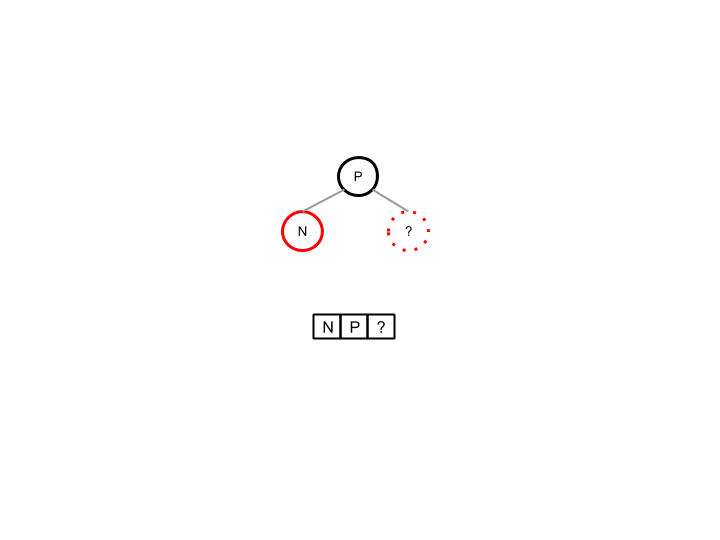
\includegraphics[scale=0.75]{pics/red_black_tree/ins_bpar}
    \caption{Insertion where $N$ has a black parent}
  \end{figure}
  \item $N$ has a red parent. This case is further divided into two cases:
  \begin{enumerate}
    \item $N$'s uncle is null. Note that $N$'s uncle cannot be black and $S$ must be a leaf, otherwise black height will not be constant. To rebalance, we simply perform an AVL rotation and recolor.
    \begin{figure}[h!]
      \centering
      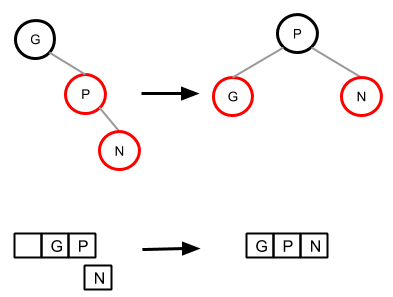
\includegraphics[scale=0.75]{pics/red_black_tree/ins_rpar_bunc_rr}
      \caption{Insertion where $N$ has a red parent and black uncle: RR rotation}
    \end{figure}
    \begin{figure}[h!]
      \centering
      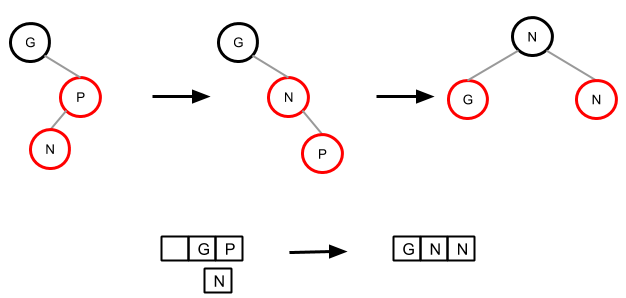
\includegraphics[scale=0.65]{pics/red_black_tree/ins_rpar_bunc_rl}
      \caption{Insertion where $N$ has a red parent and black uncle: RL rotation}
    \end{figure}
    \item $N$'s uncle is red. To rebalance, we color the parent and uncle black, color the grandparent red (if it is not the root), and then recurse on the grandparent if we created a double red. Note how this corresponds to ``pushing up'' a node in the 2-3-4 tree.
    \begin{figure}[h!]
      \centering
      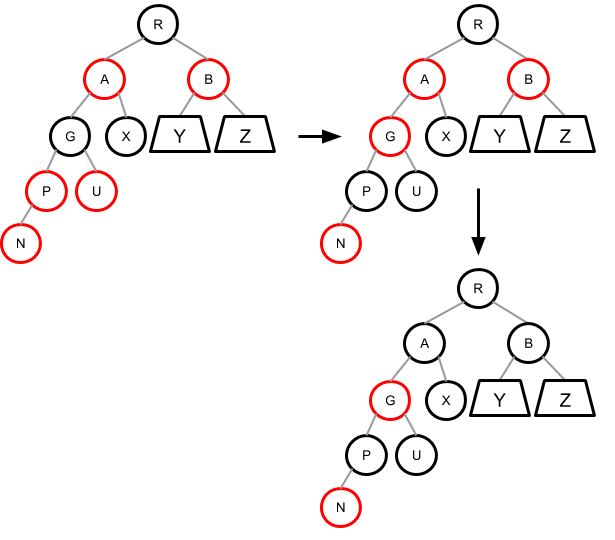
\includegraphics[scale=0.5]{pics/red_black_tree/ins_rpar_runc_rb}
      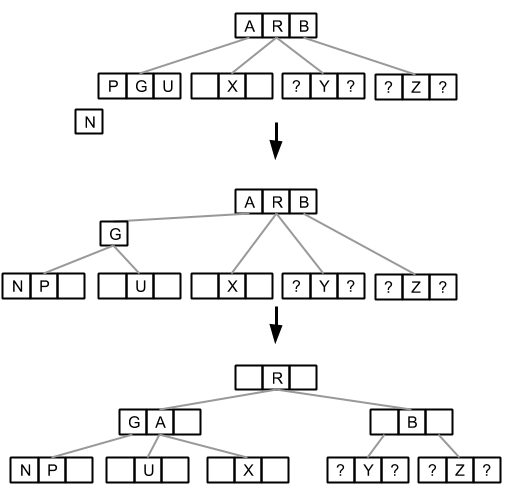
\includegraphics[scale=0.5]{pics/red_black_tree/ins_rpar_runc_234}
      \caption{Insertion where $N$ has a red parent and red uncle}
    \end{figure}

  \end{enumerate}
\end{enumerate}

%\section*{Time Complexity}

\end{document}
